\documentclass[a4paper]{IEEEtran}

  \usepackage{graphicx}
  \usepackage{hyperref}
  \usepackage{tabularx}
  \usepackage{multirow}
  \usepackage{tikz}
  \usepackage{pgfplots}
  
  \usepgfplotslibrary{statistics}
  
  \newcommand{\specialcell}[2][c]{%
  \begin{tabular}[#1]{@{}c@{}}#2\end{tabular}}
  
  \graphicspath{{illustrations/}}
  \pgfplotsset{compat=1.8}
  
  \pgfplotsset{
    /pgfplots/ybar legend/.style={
    /pgfplots/legend image code/.code={%
      \draw[##1,/tikz/.cd,yshift=-0.30em]
        (0cm,0cm) rectangle (3pt,0.8em);},
    },
  }
  
  \begin{document}
  
  \setlength{\tabcolsep}{10pt}
  \renewcommand{\arraystretch}{1.25}
  
  \begin{center}
    \textbf{\Large{
      Imagely: A cloud environment for online image processing
    }}\\
    \vspace{0.25cm}
    \emph{Authors}: SB~Ramalingam Santhanakrishnan (4740270), \\ and Z~Sun () \\
    ICT Innovation, EEMCS, TU Delft\\
    \emph{Emails}: \{S.B.RamalingamSanthanakrishnan, Z.Sun-1\}@student.tudelft.nl\\
    \vspace{0.2cm}
    \emph{Course Instructors}: Jan S. Rellermeyer,\\
    PDS Group, EEMCS, TU Delft\\
    \emph{Email}: j.s.rellermeyer@tudelft.nl@tudelft.nl\\
    \vspace{0.2cm}
    \emph{Teaching Assistants}: L~Versluis and S~Talluri,\\
    EEMCS, TU Delft\\
    \emph{Emails}: {\{L.F.D.Versluis@, S.Talluri@student\}.tudelft.nl}\\
  \end{center}
  
  \vspace{0.2cm}
  
  \textbf{
    \emph{Abstract}---\emph{Dragon Arena System} is an online multiplayer board game service designed for the specific requirements of WantGame BV. Multiple players from different locations coordinate on the virtual board to eliminate a strong AI adversary, namely the dragons. The service is hosted on Amazon Web Services (AWS) IaaS barebone compute resources, running in multiple instances to allow for scalability and fault tolerance and the system is written in NodeJS in functional reactive style. In our design, we prioritize availability and the overall responsiveness of the service while maintaining a reasonable consistency. We test the system using simulated client bots and show that the system can stay responsive under peak load to more than x\% of the clients and also analyze the fault tolerance capabilities of the system. 
  }
  
  \section{Introduction}
  
  WantGame BV is a popular online gaming company and are designing a new board game ready to roll out to multiple players. As the company is entering the rapidly expanding market of gaming, they face stiff competition and must maximize the user experience in order to survive in the industry, if not make profit. The gaming server must be able to cope up with peak traffic demands and frequent disconnections from players. Thus, WantCloud BV is evaluating several system designs for their brand new game engine, one of which is presented and analyzed in this report.
  
  The proposed system utilizes Amazon Web Services (AWS)~\cite{aws} IaaS cloud service provider's compute instance, EC2 (Elastic Cloud Compute) for providing on-demand compute capacity to host the game engine.
  Apart from using EC2, we do not depend on any other services provided by AWS so that WantGame BV can switch providers or self-host in the future. The gaming engine itself is written in NodeJS~\cite{nodejs}, on a single threaded event loop as it is a comfortable programming model for a gaming system (traditionally games have been written in while-true loops) and uses TCP/IP socket communication via websockets using the socket.io library~\cite{socket.io}. For analysis purposes, we restrict the gameplay speed to 1 second per event loop so that it is easier to compute the metrics and manually inspect the state of the system if needed. The gaming client is a small ReactJS~\cite{ReactJS} application which visualizes the board and allows keyboard inputs from the player. To simulate several players, we use client bot scripts which send simulated commands to the server, following simple strategies, events are logged both on the client and server side for later analysis.
  
  The overall system design follows master-agent\footnote{Formerly known as master-slave} architecture, where the master gets events directly from the clients and forwarded events from the agents. The master periodically broadcasts the current state of the system to all connected parties and agents forward the state to their own connected clients.

  Prior work on designing gaming systems while maintaining consistency has been done in TSS~\cite{TSS}. We have adopted ideas from TSS, mainly on the lines of TimeWarp~\cite{timewarp} to resolve late incoming events from the client that could invalidate the current state of the system. We have used disconnection log data from Game Trace Archive, specifically World of Warcraft's data and have scaled the timeline to our system for simulating client disconnection characteristics in our analysis. The goal of the test workload is to eliminate the AI units from the board.
  
  In \autoref{application}, additional background information on the application is provided. In \autoref{system_design} we illustrate the design of the system in detail with focus on specific aspects pertaining to WantGame's requirements and the rationale behind the decisions and tradeoffs that were considered. In \autoref{experiments} we present the experiments conducted along with the results and analysis. In \autoref{sec:discussion} we discuss our findings briefly and list potential improvements. We conclude the report in \autoref{conclusion} with a short summary on the main findings and recommendations to WantGame BV.
  
  \section{Application} \label{application}
  
  The online gaming server receives commands from end-users to act on their unit via the client application in a pre-agreed data protocol. The game is a 25x25 board game with two types of units, Knights (players) and Dragons (AI adversary). Knights can move, Dragons are static and the attack range is 2 squares, while the heal range is 5 squares distance, both non-diagonal distance and only Knights can heal each other. Each unit has health points and attack points, and aim to reduce the health of opponent units by attacking, which results in the opponent unit's reduction of health by the attacking unit's attack points. The system has been written in Typescript~\cite{typescript}, targeting NodeJS version 9 using ReactiveX extensions~\cite{reactivex} in the backend, the express~\cite{express} framework has been used for a tiny HTTP web server to provide an health check endpoint. The frontend and client bot have also been written in Typescript with ReactJS.
  
  \subsection{Requirements}
  
  In order to provide a reliable and interactive service, WantGame's requires the following aspects to be handled by the new system.
  
  \begin{itemize}
    \item \emph{Correct Operation}: At any point in the gameplay, the clients should see nearly consistent view of the board and actions applied on that state should be accommodated as far as possible, without violating the aforementioned rules of the game.
    \item \emph{Fault Tolerance and Availability}: The system should be resilient to failure of the clients and provide reasonable allowance for reconnection. Failure of a server instance should not result in overall seizure of the gameplay.
    \item \emph{Scalability}: The system should allow for connection of at least 100 players, supported by at least 5 functional servers.
    \item \emph{Responsiveness}: To allow for interactive gameplay, the system must remain responsive and update the board on the client as soon as the game reaches the new state.
    \item \emph{Monitoring}: At least two server instances should maintain a log of the events carried out. 
  \end{itemize}
  
  \begin{figure}[tbp]
    \centering
      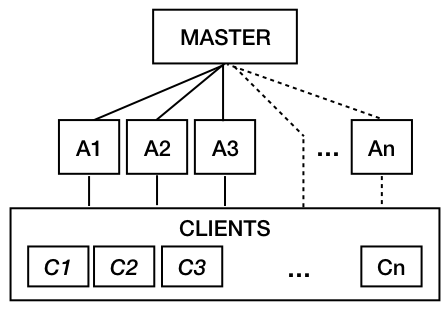
\includegraphics[width=\columnwidth]{system_design.png}
    \caption{Overview of system design.}
    \label{fig:overview_system_design}
  \end{figure}
  
  \section{System Design} \label{system_design}
  
  As mentioned in \autoref{application}, the server (master node) accepts the commands from several clients and also the forwarded commands from agents. The command is then carried out by the master at the timestamp mentioned in the command, if not too old, by going back to that state and then replaying all commands that happened on that state following the executed command. Periodically, the state updates are also sent back to the clients by the server, also forwarded by the agents. Election of the master node is out of scope of the project, however, in the system we start with a pre-selected master and a list of successors in case of failure. IN the following sections we illustrate the components of the master and the overall working of the system in terms of consistency, replication, fault-tolerance and availability.

  \subsection{Overview} \label{system_design_overview}
  
  The overall architecture of the system is illustrated in \autoref{fig:overview_system_design}, which can be seen consisting of a single master node, to which multiples agents, A1, A2, etc., are connected. Clients can connect to agents as well as the master directly, as far as the clients are concerned, the role of the server is opaque to them. Ideally, a load balancer is required in such architectures, however in this report we allow clients to randomly select servers from a known list and focus on other design aspects of the system. 
  
  The master node, illustrated in \autoref{fig:master_components} consists of the following components:
  
  \begin{itemize}
    \item \emph{Execution Queue}: The queue which maintains commands pending execution.
    \item \emph{Replay Set}: An ordered set (by timestamp) which holds the events that were previously executed, to support replays in the future. Older events in the set are periodically removed to recover memory. 
    \item \emph{Command Listener}: The socket server, which accepts client connections and subsequent commands, parses it, and adds it to the pending execution queue.
    \item \emph{Executor}: The core game engine loop present in master node which executes events in the execution queue, is invoked periodically (every 50ms in our case) and executes the event in the queue head.
    \item \emph{Forwarder}: This component runs only in agent nodes, to forward commands to the master node.
    \item \emph{Broadcaster}: Broadcast the game state periodically (every 100ms in our case) to all the connected clients and agents. 
    \item \emph{Supervisor}: Responsible for logging all the actions executed in the system, deciding weather the current node is master/agent, self-election as master and maintaining connection with master.
  \end{itemize}

  Agent nodes differ from the master node in that they have a command forwarding component instead of the executor, a state updating component connected to the master and the replay set is not utilized until it assumes leadership.
  
  \subsection{Working}
   
  \begin{figure}[bp]
    \centering
      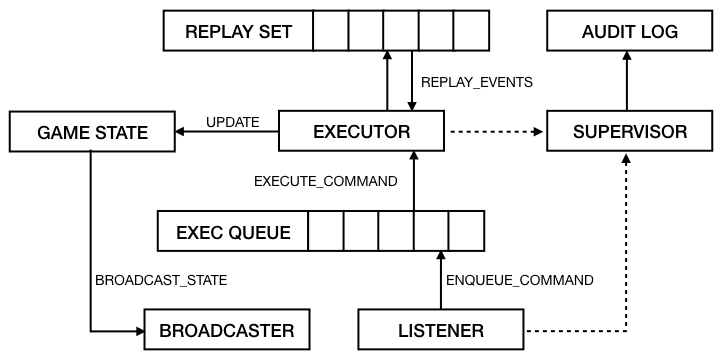
\includegraphics[width=\columnwidth]{master_components.png}
    \caption{Master components with message flows}
    \label{fig:master_components}
  \end{figure}
  
  The components in \autoref{fig:master_components} each have their own life cycle and associated events. Since we follow the reactive pattern, we illustrate the working of the system by tracing the through the execution of the system on receipt of a command from a client, through the system's various components.
  
  \begin{enumerate}
    \item \emph{Bootstrap}: This phase marks the start of the system, before the arrival of commands. The server nodes start and one of the nodes assumes leadership based on prior configuration and starts listening for client as well as agent connections. The game state consists of the board state with units and their health/attack points and also a scalar timestamp, set to 0 at the start. The timestamp is advanced on execution of each command. Agents make their connections to the master and listen for client connections as well as state updates from the master. 
  
    \item \emph{Command Receipt}: The listener listens for incoming commands from end-users and adds it to the execution queue. The executor periodically picks tasks from the execution queue, looks at the current timestamp and determines if the state for requested timestamp is present in the replay set. If not, then the command is simply discarded. If exists, then the executor picks the corresponding state from the replay set and executes all the stored commands that occurred after the given timestamp and finally updates the resultant state and also stores it in the replay state. We try to maintain weak consistency, on the assumption that most of the actions requested by the player are local to his position on the board (upto 5 squares for healing), thus limiting the chances of overwriting other parts of the board. In case there are conflicting events, then we follow the policy of last-write wins. 

    \item \emph{Monitoring}:

    \item \emph{Game State Progress}:

    \item \emph{Master Failover}:
 
  \end{enumerate}
  
  \subsection{System Capabilities \& Limitations}
  
  In this section we discuss the various tradeoffs made by the systems and its limitations.
  
  \begin{enumerate}
    \item \emph{Synchronization}: 

    \item \emph{Consistency and Replication}: 
  
    \item \emph{Fault Tolerance}: 
  \end{enumerate}
  
  \section{Experimental Results} \label{experiments}
  
  We conduct a total of n experiments and analyse the results in the following sub-sections.
  
  \subsection{Setup}
  
  The goal of the experiments is to analyse the impact of consistency and responsiveness as a function of total client connections and disconnection events. The test system is deployed on the AWS cloud platform using bare bone EC2 compute instances. We use the m3.medium type (vcpus=1, memory=3.75Gb based on Intel Xeon E5-2670 v2) for both the master and the agent nodes. We restricted the deployment to a single region, North Virginia (US-East-1) with default availability zone placement policy and the default virtual private cloud settings provided by AWS. A custom security group is used for exposing ports 80 to clients and port 8000 to agents. Health checks are done on port 80 as well via HTTP.
  
  The workload consists of upto 100 client bots and each bot is managed by a runner, which kills and spawns new bots as per the game trace archive's logs. The logs are recorded on the local AWS disk and analysed separately.
  We use python libraries pandas, scipy and numpy to analyse the time series log data and matplotlib for visualizing the same. We also run the bots on the same AWS region and availability zone subnet on a separate EC2 instance to minimize unplanned network disruptions.
  
  \subsection{Experiments}
  
  \subsubsection{Overheads}

  The latency between EC2 servers was found to be an average of x. Logging overhead was found to be y. We did not find any significant overheads that could affect the experiments on the client bot or other parts of the system.
  
  \subsubsection{Consistency Deviation}
  
  \subsubsection{Responsiveness}
  
  \subsubsection{Fault tolerance}

  \subsection{Server connection Benchmark}
  
  \section{Discussion}
  
  \label{sec:discussion}
  
  The experiments and analysis suggest that....
  
  For future work on the implementation, we would like to work and present on a more accurate time
  series analysis to trace the events and identify patterns which lead to the specific problems
  we encountered with the current system. In addition we would like to work extensively to improve in the following areas.
  
  \begin{enumerate}
    \item Master restart and detecting network partition. Currently, only fail-stop of master node is supported.
    \item Scale up and scale down server instances dynamically. This is mainly to save cost but requires a leader election algorithm in place.
    \item Implement a load balancer so that the client connections are distributed fairly and low latency servers are selected by the clients. 
    \item Build replication and synchronization for hosting multiple masters. A simple addition could be to add a master to manage a separate region of the game map.
  \end{enumerate}
  
  Clearly there are many other drawbacks in our implementation which we wish to overcome. However the experiments gave deep insights into the various tradeoffs in building a distributed system which has tight constraints on responsiveness.
  
  \section{Conclusion} \label{conclusion}
  
  In the report, we have designed and analysed a multiplayer gaming engine, aligned to the chief requirement of WantGame BV, to maintain responsiveness at peak traffic demands, which is clearly met by the system, as seen in the experimental results, where a majority of the clients are able to see their action executed in under \textbf{x} (seconds), while maintaining a consistent view of the game. The tradeoff made in fault-tolerance and scalability has to be noted though, mainly in that the system is not elastic and has to have scaling mechanism in place without disruption of gameplay. In addition we found that in some cases, optimistically processing commands in the client and agent can greatly improve the responsiveness as well as offload the master server. After analyzing the tradeoffs, we think that it is a worthy endeavour for WantGame BV to build a system with the proposed design and keep improving as new features are to be met.
  
  \bibliographystyle{myIEEEtran}
  \bibliography{report}
  
  \section*{Appendix A: Time Sheets}
  
  \begin{table}[htbp]
    \centering
    \caption{Time spent on the project per activity.}
    \begin{tabular}{| l | c |}
      \hline
      Activity & Time (hours) \\
      \hline
      Total & 170 \\
      Think & 20 \\
      Dev & 80 \\
      XP & 15 \\
      Analysis & 15 \\
      Write & 20 \\
      Wasted & 20 \\
      \hline
    \end{tabular}
  \end{table}

  \begin{table}[htbp]
    \centering
    \caption{Time spent per experiment.}
    \begin{tabular}{| l | r | r | r |}
      \hline
      & \multicolumn{3}{| c |}{Time (hours)} \\
      \hline
      & Dev & Setup & Total \\
      \hline
      Consistency Deviation & 8 & 4 & 12 \\
      Responsiveness & 1 & 0.5 & 1.5 \\
      Fault Tolerance & 1 & 0.5 & 1.5 \\
      Benchmark & 1 & 0.5 & 1.5 \\
      \hline
    \end{tabular}
  \end{table}
 
  \end{document}